\documentclass[12pt]{article}

\usepackage{geometry}
\usepackage{graphicx}
\graphicspath{ {figures/} }
\usepackage{times}
\usepackage{fancyhdr}
\usepackage{lipsum} % Used to generate random text
\usepackage{titletoc}
%\usepackage{hyperref}
%\usepackage[linktocpage=true]{hyperref}
\usepackage{setspace}
\usepackage{tocloft}
%\usepackage{etoolbox}

\usepackage{ngerman}
\usepackage{listings}
\usepackage{xcolor}

\definecolor{codegreen}{rgb}{0,0.6,0}
\definecolor{codegray}{rgb}{0.5,0.5,0.5}
\definecolor{codepurple}{rgb}{0.58,0,0.82}
\definecolor{backcolour}{rgb}{0.95,0.95,0.92}

\lstdefinestyle{mystyle}{
	backgroundcolor=\color{backcolour},   
	commentstyle=\color{codegreen},
	keywordstyle=\color{magenta},
	numberstyle=\tiny\color{codegray},
	stringstyle=\color{codepurple},
	basicstyle=\ttfamily\footnotesize,
	breakatwhitespace=false,         
	breaklines=true,                 
	captionpos=b,                    
	keepspaces=true,                 
	numbers=left,                    
	numbersep=5pt,                  
	showspaces=false,                
	showstringspaces=false,
	showtabs=false,                  
	tabsize=2
}

\lstset{style=mystyle}

% Removes paragraph indentation.
\setlength\parindent{0pt}

% Sets paper size and margins.
\geometry{
	paper=a4paper,
	top=2.5cm,
	bottom=2cm,
	left=2.75cm,
	right=2.75cm
}

% Formatting parameters for header and footer.
\pagestyle{fancy}
\fancyhf{}
\rhead{\rightmark}
\lfoot{Title of the Thesis}
\rfoot{\thepage}
\renewcommand{\headrulewidth}{0.1pt}
\renewcommand{\footrulewidth}{0.1pt}
\renewcommand\sectionmark[1]{}

% Sets counter to be used when switching page numbering roman-arabic-roman.
\newcounter{savepage}

% Formatting parameters for the table of contents.
\dottedcontents{section}[2.5em]{\bfseries}{2.5em}{0.8pc}
\dottedcontents{subsection}[2.5em]{}{2.5em}{0.8pc}

% Formatting parameters for the list of figures
\renewcommand{\thefigure}{\thesection-\arabic{figure}}
\renewcommand{\cftfignumwidth}{5em}
\renewcommand{\cftfigpresnum}{Figure }

% Formatting parameters for the list of figures
\renewcommand{\thetable}{\thesection-\arabic{table}}
\renewcommand{\cfttabnumwidth}{5em}
\renewcommand{\cfttabpresnum}{Table }

\begin{document}
% Cover page begins.
\begin{center}
	\vspace{3cm}
	\Large\textbf{Title of the Thesis}\\
	\vspace{1cm}
	\normalsize\textbf{Subtitle}
	\vspace{3cm}

%	\begin{figure}[!h]
%		\centering
%		\includegraphics[width=\textwidth]{Bar.png}
%	\end{figure}

	\begin{figure}[!h]
		\centering
		
\includegraphics[scale=0.19]{hsalbsigNAME}
		%\includegraphics[scale=0.3]{FAU.png}
	\end{figure}

	\vspace{3cm}
	\small Freie wissenschaftliche Arbeit zur Erlangung des akademischen Grades\\
	\vspace{1cm}
	\small \textit{Bachelor of Science}\\
	\vspace{1cm}
	\small an der Hochschule Albstadt-Sigmaringen\\
	\vspace{4cm}
	\line(1,0){400}
\end{center}

\begin{flushleft}
	\begin{tabular}{ll}
		Eingereicht von: & Vorname Name\\
		 & Straße Hausnummer\\
		 & PLZ Wohnort\\
		Matrikelnummer: & xxxxxxxx\\
		Studiengang: & IT Security\\
		Referent: & Prof. Dr. Freimut Bodendorf\\
		Betreuer: & M.Sc. Philipp Klinger\\
		Bearbeitungszeit: & TT.MM.2021 bis TT.MM.2021\\
	\end{tabular}
\end{flushleft}
\thispagestyle{empty}
\cleardoublepage

%% Disclaimer page begins.
%\begin{center}
%%	\begin{figure}[!h]
%%		\centering
%%		\includegraphics[scale=0.3]{FAU.png}
%%	\end{figure}
%
%	\begin{figure}[!h]
%		\centering
%		
\includegraphics[scale=0.35]{hsalbsigLOGO}
%	\end{figure}
%
%	\small Hochschule Albstadt-Sigmaringen\\
%%	\small\textit{Prof. Dr. Freimut Bodendorf}\\
%	\vspace{1cm}
%	\Large\textbf{Sperrvermerk}\\
%	\vspace{1cm}
%\end{center}
%Die Bachelorarbeit beinhaltet in Teilen interne vertrauliche Informationen der Firma xxx. Die Weitergabe des Inhaltes der Arbeit und eventuell beiliegender Zeichnungen und Daten ist untersagt. Es dürfen keinerlei Kopien oder Abschriften gefertigt werden. Ausnahmen bedürfen der Genehmigung der Firma xxx.
%\thispagestyle{empty}
%\cleardoublepage

\begin{center}
	\section*{Danksagung}
\end{center}
\markright{ } % Sets the section name to show in the header.
\vspace{1cm}
Thanks, to...
\thispagestyle{empty}
\cleardoublepage

% Adds "Page" to the table of contents.
\addtocontents{toc}{~\hfill\textbf{Page}\par}

%\makeatletter
%\patchcmd{\@fancyhead}{\rlap}{\color{red}\rlap}{}{}
%\patchcmd{\headrule}{\hrule}{\color{red}\hrule}{}{}
%\patchcmd{\@fancyfoot}{\rlap}{\color{green}\rlap}{}{}
%\patchcmd{\footrule}{\hrule}{\color{green}\hrule}{}{}
%\makeatother

\addcontentsline{toc}{section}{Kurzfassung/Abstract}
\section*{Kurzfassung}
\spacing{1.5}
\lipsum[8]
\pagenumbering{Roman}
%\cleardoublepage

\section*{Abstract}
\spacing{1.5}
\lipsum[8]
\pagenumbering{Roman}
\cleardoublepage

\addcontentsline{toc}{section}{Inhaltsverzeichnis}
\section*{Inhaltsverzeichnis}
\makeatletter
\@starttoc{toc}
\makeatother
\markright{ } % Sets the section name to show in the header.
%\cleardoublepage

%\addcontentsline{toc}{section}{\listfigurename}
%\markright{ } % Sets the section name to show in the header.
%\listoffigures
%\cleardoublepage

\cleardoublepage

\addcontentsline{toc}{section}{\listfigurename}
\section*{Abbildungsverzeichnis}
\makeatletter
\@starttoc{lof}
\makeatother
\markright{ } % Sets the section name to show in the header.
\cleardoublepage

\addcontentsline{toc}{section}{\listtablename}
\section*{Tabellenverzeichnis}
\makeatletter
\@starttoc{lot}
\makeatother
\markright{ } % Sets the section name to show in the header.
\cleardoublepage

\addcontentsline{toc}{section}{Abkürzungsverzeichnis}
\section*{Abkürzungsverzeichnis}
\makeatletter
\@starttoc{lot}
\makeatother
\markright{ } % Sets the section name to show in the header.
	\vspace{1cm}
	\begin{tabular}{lcl}
		\textbf{CPU} & & Central Processing Unit\\
		&&\\
		\textbf{PC} & & Personal Computer\\
	\end{tabular}
\cleardoublepage

\section{Kapitel 1 - Grundlagen}
\markright{Introduction} % Sets the section name to show in the header.
\setcounter{savepage}{\arabic{page}}
\pagenumbering{arabic}
\lipsum[1-2]
\begin{figure}[!h]
	\centering
	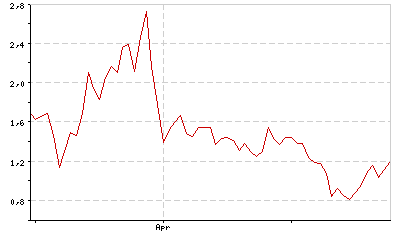
\includegraphics[scale=1.0]{Graph.png}
	\caption[A nice graph.]{A nice graph representing a measure. Source (XXX)}
	%\caption{A nice graph.}
\end{figure}
\cleardoublepage

\section{Kapitel 2 - Multithreading/processing}
\markright{Second Section} % Sets the section name to show in the header.
\setcounter{figure}{0} % Restarts the figure counting.
\setcounter{table}{0} % Restarts the table counting.
\lipsum[1]
\begin{figure}[!h]
	\centering
	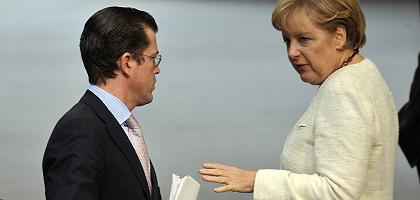
\includegraphics[scale=1.0]{Merkel.png}
	\caption[A. Merkel]{Angela Merkel in action. Source (YYY)}
\end{figure}
\lipsum[2]
\subsection{First Subsection}
\lipsum[3]
\subsection{Second Subsection}
\lipsum[4]
\begin{table}
	\centering
	\begin{tabular}{| l c r |}
		\hline
		1 & 2 & 3 \\
		4 & 5 & 6 \\
		7 & 8 & 9 \\
		\hline
	\end{tabular}
	\caption{A simple table}
\end{table}
\lipsum[2]
\cleardoublepage

\section{Kapitel 3 - GUI-Ergänzung}
\lipsum[3]
\cleardoublepage

\section{Kapitel 4 - Debugging Modus}
\lipsum[3]
\cleardoublepage

\section{Kapitel 5 - Tests der Ergebnisse einer ausgewählten Forensik Suite}
\lipsum[3]
\cleardoublepage

\section{Kapitel 6 - Unittests(?)}
\lipsum[3]
\cleardoublepage

\section{Kapitel 7 - Fazit}
\lipsum[9]
\lipsum[8]
\lipsum[8]
\lipsum[3]

Durch die überlappenden CPU-intensiven Tasks wird eine scheinbar parallele Ausführung möglich. Jedoch ist diese immer von der Schnelligkeit von I/O-abhängigen (I/O-Bound) Lese- und Schreibvorgängen und den Freigaben des GIL abhängig. 
Beim Multiprocessing dagegen ist kein „Global Interpreter Lock“ notwendig, da jeder Process seinen eigenen Speicherbereich besitzt. Speicherbereiche müssen nicht extra blockiert und freigegeben werden.
(Indirekte Quelle für dieses Wissen: ein Buch?)
Die Überlegung der Machbarkeitsstudie besteht darin, zu überprüfen, ob anhand von Multithreading/Multiprocessing die Perfomance des Ladevorgangs von Browserprofilen im Vergleich zur normalen Ausführung, ohne mehrere parallel ablaufende Tasks, be-schleunigt werden kann?
Zunächst wird das Auslesen einer SQLite-Datenbank unter möglichst denselben Um-gebungsbedingen getestet. 
Dabei wird die PoC Software in der identischen Entwicklungsumgebung auf dem glei-chen Testsystem (siehe Komponentenliste) in Verbindung mit der identischen SQLite-Datenbankdatei, durchgeführt. Die Tests erfolgen hintereinander.
Es wird eine Programm-Variante des PoC ohne Multithreading mit einer Variante mit Multithreading und unterschiedlichen Anzahlen von Threads verglichen. 
Dabei wird der Fokus vor allem auf den Test mit einer großen SQLite-Datenbank ge-legt.\\

Komponenten und Betriebssystem des Testsystems:
\begin{itemize}
	\item Processor	Intel(R) Core (TM) i9-9900K CPU @ 3.60GHz,\\
	3600 MHz, 8 Core(s), 16 Logical Processor(s)
	\item Installed Physical Memory (RAM)	32.0 GB
	\item OS Name	Microsoft Windows 10 Home
	\item Version	10.0.19043 Build 19043
\end{itemize}
	
Die Machbarkeitsstudie soll nur mit einem Browser durchgeführt werden, da die Logik hinter dem Zugriff auf SQLite-Datenbankdateien sich nur in der Datenbankdatei 
Struktur (Namensgebungen, Tabellenstrukturen) aber nicht in der Technologie unterscheidet. Der erste Versuch wurde mit dem Mozilla Firefox Browser durchgeführt. 
Allerdings ergaben sich Schwierigkeiten in dem Skript, die den Proof of Concept unnötig kompliziert werden ließen. Bei der Änderung auf den Google Chrome Browser ent-fielen diese Programmabschnitte und die Machbarkeitsstudie wurde dadurch leichter verständlich.

Reproduzierbarkeit der verwendeten SQLite-Datenbankdatei:

\lstinputlisting[language=Python]{chromeHistoryGenerator.py}

\cleardoublepage

\addcontentsline{toc}{section}{Literaturverzeichnis}
\section*{Literaturverzeichnis}
\markright{ } % Sets the section name to show in the header.
\pagenumbering{Roman}
\setcounter{page}{\thesavepage}
\lipsum[1]
\cleardoublepage

\addcontentsline{toc}{section}{Annex A}
\section*{Annex A}
\markright{Annex A} % Sets the section name to show in the header.
%\pagenumbering{Roman}
%\setcounter{page}{\thesavepage}
\lipsum[5]
\cleardoublepage

\addcontentsline{toc}{section}{Annex B}
\section*{Annex B}
\markright{Annex B} % Sets the section name to show in the header.
\lipsum[6]
\cleardoublepage

\addcontentsline{toc}{section}{Eidesstattliche Erklärung}
\section*{Eidesstattliche Erklärung}
\markright{ } % Sets the section name to show in the header.
\vspace{2cm}
Ich versichere, dass ich die Arbeit ohne fremde Hilfe und ohne Benutzung anderer als der angegebenen Quellen angefertigt habe.  Die Arbeit wurde in gleicher oder ähnlicher Form noch keiner anderen Prüfungsbehörde vorgelegt  und von dieser als Teil einer Prüfungsleis-tung angenommen. Alle Ausführungen, die wörtlich oder sinngemäß übernommen wurden, sind als solche gekennzeichnet.\\
\vspace{2cm}

\begin{flushleft}
	Nuernberg, den 7. Maerz 2017\\
	\vspace{3cm}
	\line(1,0){150}\\
\end{flushleft}
Vorname Name
\cleardoublepage

\end{document}
